\section{Results}\label{sec:results}

\subsection{Analysis}

All the analysis simulation where done with the timesteps given in \eqref{eq:timestep_set}. 

\begin{equation}\label{eq:timestep_set}
	h \in \{ 0.5, 0.3, 0.1, 0.08, 0.05, 0.01\}
\end{equation}

\subsubsection{Conservation of Energy}\label{sec:energy_conservation}

To study the differences of the integrators must a system first be chosen, in the sense that a set of initial conditions must be chosen for all the integrators. The system of choice is

\begin{equation}
	v = 0.375 , \quad M = 1, \quad r_0 = 10M
\end{equation}

where we so far does not have to define the units (this will be done for the Mercury orbit simulation though). 

\begin{figure}[ht!]
	\centering
	\includegraphics[width=0.8\textwidth]{figures/energy_conservation/euler.png}
	\caption{Results for Euler Method. Above is the energy vs. the time, while below is the radius compared to the time. }
	\label{fig:euler_energy_cons}
\end{figure}
\begin{figure}[ht!]
	\centering
	\includegraphics[width=0.8\textwidth]{figures/energy_conservation/back_euler.png}
	\caption{Results for Backward Euler. Above is the energy vs. the time, while below is the radius compared to the time. }
	\label{fig:back_euler_energy_cons}
\end{figure}
\begin{figure}[ht!]
	\centering
	\includegraphics[width=0.8\textwidth]{figures/energy_conservation/rk4.png}
	\caption{Results for RK4. Above is the energy vs. the time, while below is the radius compared to the time. The different radius plots are perfectly aligned here, which is why there is only one plot evident. }
	\label{fig:rk4_energy_cons}
\end{figure}

Firstly studying the Euler method, we can see in \ref{fig:euler_energy_cons} that the energy decreases in time in a linear fashion. Note also that the slope depends on the timestep, with smaller timesteps corresponds to better energy conservation and vice versa. The energy loss can also be seen in the coordinates of the result, where the radius of the orbit slowly decays as both the peaks and valleys of the radius decreases with time. 

Continuing to the Backward Euler results, there is an exponential decay evident in the energy plots in fig. \ref{fig:back_euler_energy_cons}. Compared to the Euler method results doe the energy here decay much faster (by comparing the energy ranges on the y-axis), but it at least (seemingly) converges in contrast to the linear decay for Euler. When also studying the radius plotted against time, we see that the amplitude of the oscillations is dampened, but the mean is seemingly conserved. For orbital mechanics is this a bad property, as it is not expected for the amplitude to be dampened. 

Finally, studying the results of RK4 in fig. \ref{fig:rk4_energy_cons}, there is a slight increase in energy appearent for $h = 0.5$. However, note that the energy varies on a scale of the order of magnintude of $10e-12$, which in comparison to the other integrators' results are insignificant variations and is hence practically static. It can be further observed that the RK4 integrations of different timestep corresponds to the same solutions. 

With regards to energy conservation does RK4 outperform the other two integrators by a large margin, while Euler performs better than Backward Euler slightly. The latter observation is interesting, since it is widely regarded that Backward Euler is more roboust than regular Euler. 

\subsubsection{Error compared to analytical solution}

When setting the initial velocity of the orbiting mass to $v = \sqrt{M / r}$ will the resulting orbit be perfectly circular. When setting these initial condition for all of the integrators and comparing to the static radius (set to $10$), the integrators solves the equations perfectly. 

\begin{table}[!ht]
	\centering
	\caption{Results of the integrators for circular orbit initial condition. The numbers shown are exact (up to computers margin of error). }
	\label{tab:analytical_comp}

	\begin{tabular}{|c|c|c|c|c|c|c|}
		\hline
		$h$ & \multicolumn{6}{|c|}{Integrators, avg. and var. alternating} \\ \hline
		    & \multicolumn{2}{|c|}{Euler} & \multicolumn{2}{|c|}{Backward Euler} & \multicolumn{2}{|c|}{RK4} \\ \hline
		1.5 & 10.0 & 0.0 & 10.0 & 0.0 & 10.0 & 0.0 \\ \hline
		1.3 & 10.0 & 0.0 & 10.0 & 0.0 & 10.0 & 0.0 \\ \hline
		1.1 & 10.0 & 0.0 & 10.0 & 0.0 & 10.0 & 0.0 \\ \hline
		1.08 & 10.0 & 0.0 & 10.0 & 0.0 & 10.0 & 0.0 \\ \hline
		1.05 & 10.0 & 0.0 & 10.0 & 0.0 & 10.0 & 0.0 \\ \hline
		1.01 & 10.0 & 0.0 & 10.0 & 0.0 & 10.0 & 0.0 \\ \hline
	\end{tabular}
\end{table}

The results are thus trivial and does not show any differences over the different integrators tab. \ref{tab:analytical_comp}. They perfectly align with the analytical solution. 

\subsubsection{Perihelion precession error}\label{sec:precession_analysis}

\begin{figure}[!ht]
	\centering
	\begin{subfigure}[h!]{0.3\textwidth}
		\centering
		\includegraphics[width=\textwidth]{figures/precession_analysis/euler.png}
		\caption{Orbit precession change for Euler integrator in units of $\pi$ radians. }
		\label{fig:euler_precession_analysis}
	\end{subfigure}
	\hfill	
	\begin{subfigure}[h!]{0.3\textwidth}
		\centering
		\includegraphics[width=\textwidth]{figures/precession_analysis/back_euler.png}
		\caption{Orbit precession change for Backward Euler integrator in units of $\pi$ radians.}
		\label{fig:back_euler_precession_analysis}
	\end{subfigure}
	\hfill
	\begin{subfigure}[h!]{0.3\textwidth}
		\centering
		\includegraphics[width=\textwidth]{figures/precession_analysis/rk4.png}
		\caption{Orbit precession change for RK4 integrator in units of $\pi$ radians. } 
		\label{fig:rk4_precession_analysis}
	\end{subfigure}
	\caption{The precession of each the orbit completed plotted against the timestep parameter. The precession generally increases for each completed orbit. }
	\label{fig:precession_analysis}
\end{figure}

Studying the orbit precessions in fig. \ref{fig:precession_analysis}, there are some resemblences as well as differences. What all the methods do is converge towards a specific value for the orbit precession, a value that is around $0.68$. However, there is a difference iin how the methods converge to the precession value (and exactly what this convergent value is). In \ref{fig:euler_precession_analysis}, there is a linear convergence as the time step with decreasing timestep. Backward Euler in \ref{fig:back_euler_precession_analysis} on the contrary shows more of a quadratic relationship, and finally RK4 fig. \ref{fig:rk4_precession_analysis} has a more erratic pattern but not the less convergent. 

Another pattern for the three integrators is that the variance increases with the increase of the timestep parameter. This means that for larger time steps will the precession become larger and larger for each orbit completed, which can also be seen in the radius plot for Euler most prominently \ref{fig:euler_energy_cons}. 

Although the way the integrators' precession converge is of importance, the scale at which these different results live in is more vital. The Euler method only has an margin of error in the ranges of the first decimal place. This increases to the second decimal place for Backward Euler and lastly to the third for RK4. Having this in mind, one can argue that RK4 performs the best, as the difference between the precessions over the different completed orbits is minimal (two orders of magnitude less then what the precession converges to). 



\subsection{Orbit of Mercury}

In order to correctly model the orbit of Mercury, we have to introduce a set of units that are representative of the scale at which the physics is happening. In order to do this we ibegin to study the equations the systems obeys \eqref{eq:eoms}. Here we have set the speed of light to 1, which effectively means that mass and length have the same dimension: $[M] = [r] = \text{length}$ (this fact can be seen in the metric of the system \eqref{eq:schwarzschild-metric}, where the dimensionless terms have a fraction of mass and distance which implies that both must have the same unit). Furthermore, the mass of the sun is on the scale of $10^{30}$ kg, while the typical distance in the solar system is about $10^9$ m, this means that we simply cannot rescale both the quantities with the same factor. We begin to define the length and time scale that we want. 

As stated before, the typical scale at which the solar system dynamics takes place is on about 1 astronomical unit (\si{au}) (Mercury orbits on around 0.3-0.4 \si{au}), and orbits takes around 100s of days (Eartly days) to complete, hence is it suitable to convert the time from seconds to days. In order to convert the mass from kgs to au (which is now used in the equations), we need to utilize the gravitational constant $G$. 

\begin{table}[!h]
	\centering
	\begin{tabular}{|c|c|}
		\hline 	 
		Constant 	& Value and unit \\ 					\hline
		$G$ 		& \num{6.67430e-11} 	\si{m^3.kg^{-1}.s^{-2}} \\	\hline
		$R_0$ 		& \num{149 597 871} 	\si{km.au^{-1}} \\		\hline
		$T_0$		& \num{86400} 		\si{s.day^{-1}}	\\		\hline
	\end{tabular}
	\caption{The relevant constants (with units) defined. }
	\label{tab:conversions}
\end{table}

By using the constants defined in tab. \ref{tab:conversions}, we can obtain the length-united mass through the relation

\begin{equation}\label{eq:mass_conversion}
	M = \frac{G T_0^2}{R_0^3} M_\text{kg}
\end{equation}

Using parameters given from \cite{nasa_mercury,wiki_sun} given in tab. \ref{tab:mercury_parameters}, we can set the initial conditions for the simulation. We choose the perihelios to be the initial radius, at the point of which which the velocity is the greatest. Furthermore, we can convert the Solar mass to our choice of units with the conversion units.  

\begin{table}[!ht]
	\centering
	\begin{tabular}{|c|c|}
		\hline
		$r_{\text{perihelios}}$ &  \num{0.3075}	\si{au}			\\ 	\hline
		$r_{\text{aphelios}}$ 	&  \num{0.4667} \si{au} 		\\ 	\hline
		$v_{\text{minimum}}$	&  \num{0.03406} \si{au.day^{-1}}	\\	\hline
		$M_{\si{kg}}$		& \num{	1.9885e30} \si{kg}		\\ 	\hline	
		$M$			& \num{	2.9592e-4} \si{au}		\\ 	\hline	
	\end{tabular}
	\caption{The relevant parameters for the simulation of the Mercury orbit.}
	\label{tab:mercury_parameters}
\end{table}

The simulation was done for 1000 days, using the timestep $h = 0.001$ for each integrator. 

\begin{figure}[!ht]
	\centering
	\includegraphics[width=0.8\textwidth]{figures/mercury_solution.png}
	\caption{Solutions for the Mercury orbit. Above is the full solution, and below is a zoomed in view on the last simulated aphelion (largest radius). Furthermore is the aphelion and perihelion marked with the black lines. }
	\label{fig:mercury_result}
\end{figure}

Observing the results in \ref{fig:mercury_result}, we notice some interesting results. Firstly, the three integrators are very similar in their solutions. By their last completed orbit a small difference be seen, largely a difference in precession. Furthermore, more interestingly, are the simulated aphelions around $0.01 au$ away from  observed values, which is consitent for all the integrators, while the perihelion distance stays practically the same. 

\begin{table}[ht]
	\centering
	\begin{tabular}{|c|c|c|c|c|c|}
		\hline
						& Euler 	& Backward Euler 	& RK4 		& Prev. established values 	\\ \hline
		Orbit time, avg [day]		&$89.38$		&$89.44$ 		&$89.42$		&$87.97$		\\ \hline
		Orbit time, var [day]		&\num{3.18e-4}		& \num{1.48e-4}	 	&\num{9.00e-8}		&			\\ \hline
		Precession per century [rad]	&\num{-26.41}		&\num{-26.38}  		&\num{-26.37}		&\num{2.036e-4}		\\ \hline
		Aphelion [au]			&\num{0.47813}		&\num{0.47849} 		&\num{0.47816}		&\num{0.46670}		\\ \hline
		Perihelion [au]			&\num{0.3073}		&\num{0.3073} 		&\num{0.3075}		&\num{0.30749}		\\ \hline
	\end{tabular}
	\caption{Results of the simulation compared to observed values and other calculations. The calculated perihelion precession from \cite{wiki_precession} is only accounting for relativistic effects. } %\cite{nasa_mercury, wiki_precession}. }
	\label{tab:results}
\end{table}



Taking a closer look on our results in tab. \ref{tab:results} (obsered values are taken from \cite{nasa_mercury, wiki_precession}) we see that even though the aphelion overshoots by \num{0.01} \si{au}, the orbit time for all the integrators only overshoots by approximately 1 day! 

However, the most striking difference between the simulated values and the observed values is the precession, which are firstly negative, and secondly 6 magnitudes larger that that of the observed precession. This is a large discrapency, as is the aphelion, which leads us to believe that these could be connected. 




